\chapter{Przeniesienie obliczeń fizycznych na procesor karty graficznej}

Niniejszy rozdział prezentuje techniki zastosowane w celu przeniesienia głównych
obliczeń fizycznych na kartę graficzną w symulatorze Energy2D będącym
przedmiotem tej pracy. Na początku opisane są tradycyjne podejścia do tego
problemu dla aplikacji działających w natywnym środowisku systemu operacyjnego
oraz ich odniesienie do środowiska oferowanego przez przeglądarki internetowe.
Następnie zaprezentowana jest technologia \mbox{WebGL} dzięki której dokonano
właściwego zrównoleglenia obliczeń symulatora. W ostatnim podrozdziale opisana
została właściwa implementacja. Informacje te mogą być szczególnie użyteczne
przy próbach podobnych optymalizacji innych aplikacji.

Dzięki przeniesieniu obliczeń fizycznych na GPU uzyskano istotny wzrost
wydajności. Dokładna analiza zysków ze zrównoleglenia symulacji jest tematyką
kolejnego rozdziału [TODO: podać dokładny rozdział].

\section{Typowe metody przenoszenia obliczeń na GPU, a przeglądarka internetowa}

Współczesna karty graficzne posiadają ogromną moc obliczeniową -- wielokrotnie
większą od centralnego procesora przy założeniu, że obliczenia da się wykonywać
w sposób równoległy. Pomysł aby przenieść część obliczeń ogólnego zastosowania
na kartę graficzną pojawił się wraz z dynamicznym rozwojem procesorów
graficznych. Szczególnie istotnym momentem było wprowadzenie programowalnych
jednostek cieniujących (specyfikacja \emph{DirectX 8}). Dalszy rozwój obliczeń
ogólnego zastosowania na kartach graficznych (ang. \emph {General-purpose
computing on graphics processing units}, w skrócie GPGPU) miał miejsce wraz z
wprowadzeniem technologii, które ukryły złożoność dostępu do zasobów karty
graficznej i udostępniły interfejs wysokiego poziomu. Wiodącymi technologiami
tego typu są \emph{OpenCL} (rozwiązanie otwarte) oraz \emph{CUDA} (zamknięte
rozwiązanie firmy NVIDIA, działające wyłącznie na sprzęcie tego producenta).

Wspomniane powyżej technologie dotyczą oczywiście aplikacji pisanych w natywnym
środowisku systemu operacyjnego. Aby programować jednostki cieniujące wystarczy
podstawowy dostęp do standardowego interfejsu OpenGL bądź Direct3D.
Implementacje tych interfejsów można znaleźć dla prawie każdego współczesnego
języka programowania. Interfejsy wyższego poziomu (OpenCL, CUDA) również
posiadają implementacje w różnych językach programowania, choć najczęstszym
środowiskiem ich działania są aplikacje napisane w C bądź C++.

Poniżej krótko przedstawione są sposoby przeprowadzania obliczeń ogólnego
zastosowania na kartach graficznych oraz ich związek ze specyficznym
środowiskiem przeglądarki internetowej.

\subsection{Niskopoziomowe programowanie jednostek cieniujących}
\label{subsec:niskProgJedn}

Jest to najstarsze podejście do przeprowadzania obliczeń ogólnego zastosowania
na procesorze karty graficznej. Programista w swoisty sposób ,,oszukuje'' kartę
graficzną, przeprowadzając renderowanie prostej geometrii wyłącznie w celu
uruchomienia własnych programów jednostek cieniujących, które wykonują
obliczenia często nie mające nic wspólnego z generowaniem obrazu.

Takie podejście jednak jest wymagające i obarczone pewnymi problemami. Łatwo
popełnić błędy, wymagana jest też przynajmniej podstawowa wiedza o
programowaniu grafiki trójwymiarowej.

\subsection{Technologie wyższego poziomu}
\label{subsec:techWyzPoz}

Technologie, które przyczyniły się do gwałtownego wzrostu popularności obliczeń
na kartach graficznych to szczególnie \emph{OpenCL} oraz \emph{CUDA}.
Udostępniają  one znacznie wyższy poziom abstrakcji -- programista jest
zwolniony z obowiązku przyswojenia sobie niskopoziomowych mechanizmów rządzących
działaniem kart graficznych (choć ta wiedza pozwala tworzyć aplikacje
efektywniejsze). Udostępniony jest specjalny interfejs oraz składnia, co
znacznie ułatwia pracę, szczególnie programistom bez doświadczenia w pracy z
programowaniem grafiki trójwymiarowej.

\subsection{Środowisko przeglądarki internetowej}
\label{subsec:srodPrzegInt}

Należy uściślić, że ,,środowisku przeglądarki internetowej'' to zbiór możliwości
nowoczesnych, wiodących przeglądarek internetowych, rozpowszechniony na tyle,
aby był dostępny dla większości użytkowników internetu. Równocześnie możliwości
te nie mogą wymagać instalowania żadnych dodatków i rozszerzeń, gdyż znacznie
ogranicza to ich dostępność. Jest to szczególnie istotne dla aplikacji
edukacyjnych, które wymagają łatwego i powszechnego dostępu.

Przeglądarka internetowa z założenia jest środowiskiem bardzo ograniczonym,
przede wszystkim ze względów bezpieczeństwa. Jednak niedawno, wraz z nadejściem
standardu HTML5, został dodany podstawowy dostęp do zasobów karty graficznej.
Realizuje go technologia WebGL, która jest implementacją standardu OpenGL ES
2.0. Tym samym pojawiła się możliwość programowania jednostek cieniujących kart
graficznych, a więc i przeprowadzania na nich obliczeń ogólnego zastosowania
(\ref{subsec:niskProgJedn}).

Technologie programowania kart graficznych wyższego poziomu
(\ref{subsec:techWyzPoz}) nie są (jeszcze) dostępne w środowisku przeglądarki
internetowej. Aktualnie trwają intensywne prace nad implementacją standardu
OpenCL o roboczej nazwie WebCL. Jednak technologia ta w aktualnym momencie jest
na bardzo wczesnym etapie rozwoju. Więcej informacji można znaleźć na stronie
internetowej: http://www.khronos.org/webcl/.


\section{WebGL -- otwarcie dostępu do zasobów karty graficznej w przeglądarce}

[TODO: opis WebGLa]

\section{Implementacji silników fizycznych Energy2D przy użyciu WebGL}

Symulator Energy2D składa się z dwóch kluczowych silników fizycznych -
przewodnictwa cieplnego oraz dynamiki płynów. Są one dokładnie przybliżone w
rozdziale [TODO: podać rozdział]. Oba te silniki są niezwykle wymagające
obliczeniowo. Dlatego też ich optymalizacja była zadaniem kluczowym, aby
stworzyć aplikację wartościową edukacyjnie. Zbyt wolny przebieg symulacji może
skutecznie zniechęcić większość potencjalnych użytkowników. Jednym z
podstawowych wymagań było, aby wirtualne laboratorium było aplikacją w pełni
interaktywną czyli również działającą jak najpłynniej.

Analiza silników fizycznych Energy2D wykazała, że nie ma przeciwwskazań aby je
zrównoleglić. Obliczenia wykonywane są na prostokątnych siatkach, nie są również
zależne od sekwencji wykonywania. Wymagane były tylko drobne modyfikacje
algorytmów rozwiązywania układów równań liniowych.

Poniżej przedstawione są najważniejsze zagadnienia związanie z przeniesieniem
obliczeń fizycznych Energy2D na kartę graficzną.

\subsection{Podstawowy zarys implementacji}

Zgodnie z wnioskami sekcji \ref{subsec:srodPrzegInt}, ze względu na ograniczenia
środowiska przeglądarki internetowej, wymuszona została implementacja
niskopoziomowa przy użyciu technologii WebGL. Opiera się ona na programowaniu
jednostek cieniujących karty graficznej, głównie wykorzystując programy
fragmentów (ang. fragment shaders).

\subsubsection{Organizacja danych w pamięci karty graficznej}

Dane symulacji (takie jak np. macierz temperatury czy macierz prędkości płynu)
przechowywane są w dwuwymiarowych teksturach zmiennoprzecinkowych. Tego typu
tekstury nie wchodzą w skład podstawowej specyfikacji WebGL 1.0
(\cite{WebGLSpec}). W związku z tym wymagane jest użycie rozszerzenia
\emph{\mbox{OES\_texture\_float}}, które jest dostępne na większości
współczesnych urządzeń ([TODO: wspomnieć o rozdziale z testami]).

Niezwykle ważną kwestią jest organizacja danych w teksturze. Jest sporo
możliwości ponieważ tekstura z zasady nie jest wierną kopią dwuwymiarowej
tablicy JavaScript, a obiektem przystosowanym do przechowywania obrazów. Stąd
posiada na przykład kanały kolorów. Programista ma jednak możliwość
konfiguracji, stąd można rozważyć kilka potencjalnych sposób na organizację
danych.

\begin{itemize}

\item Schemat 1. -- tekstury jednokanałowe (format ALPHA lub LUMINANCE), jedna
tekstura odpowiada jednej tablicy JavaScript. Dalej nazywany schematem
\textbf{A1} na potrzeby niniejszego opracowania.

\item Schemat 2. -- tekstury czterokanałowe (format RGBA), dane tylko w jednym
kanale, jedna tekstura odpowiada jednej tablicy JavaScript. Dalej nazywany
schematem \textbf{RGBA1} na potrzeby niniejszego opracowania.

\item Schemat 3. -- tekstury czterokanałowe (format RGBA) dane w każdym z
kanałów, jedna tekstura odpowiada czterem tablicom JavaScript. Dalej nazywany
schematem \textbf{RGBA4} na potrzeby niniejszego opracowania.

\item Schemat 4. -- tekstury czterokanałowe (format RGBA), dane w każdym z
kanałów, jedna tekstura odpowiada jednej tablicy JavaScript, rozmiar tekstury
zredukowany czterokrotnie, gdyż każdy kanał odpowiada jednej ćwiartce tablicy.
Dalej nazywany schematem \textbf{RGBA1/4} na potrzeby niniejszego opracowania.

\end{itemize}

Każdy z powyższych schematów został przetestowany podczas implementacji
symulatora Energy2D. Wyniki testów wydajnościowych przedstawia wykres
\ref{fig:texPerf}.

\begin{figure}[hbp]
\centering
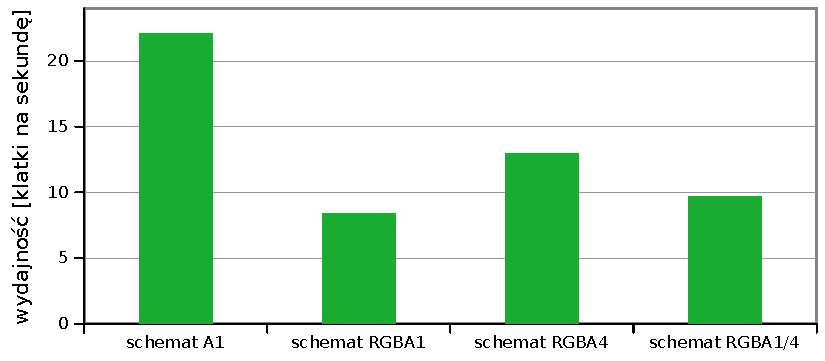
\includegraphics[width=.9\textwidth]{img/texPerf}
\caption{Wpływ organizacji danych w teksturach na wydajność symulacji Energy2D}
\label{fig:texPerf}
\end{figure}

Rozwiązaniem optymalnym ze względu na wydajność oraz czytelność kodu wydaje się
schemat A1. Umożliwia on przeniesienie danych z tablic w relacji 1:1 do tekstur.
Do tego, każdy odczyt czy zapis do tekstury dotyczy tylko jednego kanału.
Niestety, na większości urządzeń nie ma możliwości dołączenia tekstury typu
ALPHA lub LUMINANCE do własnego obiektu bufora ramki (ang. FrameBuffer Object)
-- czyli renderowania do takiej tekstury. Wyklucza to możliwość użycia tego
rozwiązania mimo oczywistych zalet. Być może w przyszłości rozwój specyfikacji
WebGL na to pozwoli.

Warto tutaj nadmienić, że specyfikacja WebGL (\cite{WebGLSpec}) nie gwarantuje,
iż jakikolwiek z formatów tekstur zmiennoprzecinkowych będzie zaakceptowany jako
cel renderowania. Programista powinien wykonać test, aby sprawdzić czy maszyna
użytkownika wspiera daną konfigurację. Można to zrobić w następujący sposób:

\begin{lstlisting}[caption=Weryfikacja poprawności formatu i typu tekstury
używanej jako cel renderowania]
var gl 		= getWebGLContext(),
	texture = gl.createTexture(),
	fbo 	= gl.createFramebuffer();

if (!gl.getExtension('OES_texture_float')) {
	throw new Error("Rozszerzenie OES_texture_float niedostępne.");
}
gl.bindTexture(gl.TEXTURE_2D, texture);
gl.texImage2D(gl.TEXTURE_2D, 0, gl.RGBA, 128, 128, 0, gl.RGBA, gl.FLOAT, null);
gl.bindFramebuffer(gl.FRAMEBUFFER, fbo);
gl.framebufferTexture2D(gl.FRAMEBUFFER, gl.COLOR_ATTACHMENT0, gl.TEXTURE_2D, 
	texture, 0);
if (gl.checkFramebufferStatus(gl.FRAMEBUFFER) !== gl.FRAMEBUFFER_COMPLETE) {
	throw new Error("Dana tekstura nie jest wspierana jako cel renderowania.");
}
\end{lstlisting}

W praktyce tekstury zmiennoprzecinkowe posiadające cztery kanały kolorów są
najczęściej akceptowanym formatem do którego można zapisywać dane podczas
renderowania. Dlatego też schematy organizacji danych RGBA1, RGBA4 oraz RGBA1/4
używają takiego formatu tekstury.

Schemat RGBA1 posiada te same zalety co A1 jeśli chodzi o organizacje i
czytelność kodu źródłowego, jednak w tym przypadku dochodzi do dużego narzutu
wydajności związanego z odczytem i zapisem tekstur. Przy każdej z tych operacji
karta graficzna musi odczytać cztery kanały, jednak praktycznie wykorzystywany
jest tylko jeden z nich. Operacje dostępu do pamięci są czasochłonne, dlatego
też taka organizacja danych nie jest korzystna ze względów wydajnościowych.

Rozwiązaniem tego problemu są schematy RGBA4 oraz RGBA1/4. Organizacja danych
wg. trzeciego schematu pozwala zredukować narzut związany z odczytem oraz
zapisem pod warunkiem dobrej organizacji danych w teksturach. Pomysł ten
obrazuje diagram \ref{fig:rgba4Tex}. 

\begin{figure}[hbp]
\centering
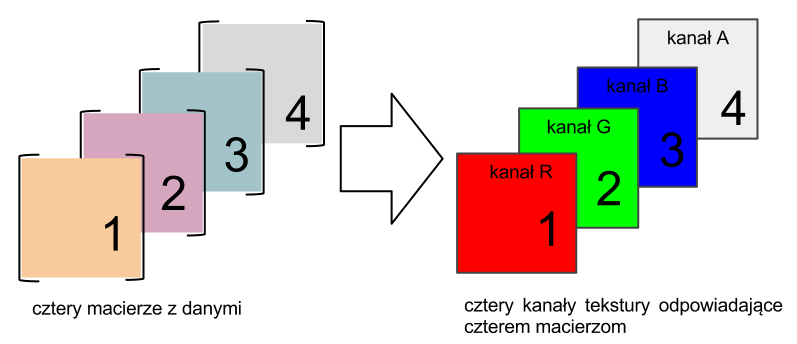
\includegraphics[width=.9\textwidth]{img/rgba4Tex}
\caption{Schemat organizacji danych z czterech macierzy w jednej teksturze}
\label{fig:rgba4Tex}
\end{figure}

Przy korzystnym ułożeniu danych jest możliwe praktycznie całkowite zredukowanie
narzutu związanego z odczytem wszystkich czterech kanałów tekstury, jednak w
praktyce jest to często niewykonalne. Przez korzystne rozmieszczenie danych
przyjmuje się takie ich ułożenie, żeby program jednostek cieniujących odczytując
teksturę faktycznie korzystał z danych zawartych w każdym z kanałów. Podobnie
przy zapisie, program renderujący powinien modyfikować wszystkie cztery kanały.
W przypadku symulatora Energy2D udało się uzyskać taką organizację danych, żeby
odczyt był w znacznym stopniu zoptymalizowany, jednak podczas zapisu
modyfikowany był tylko jeden lub dwa kanały (kanał zawierający dane o
temperaturze lub kanały zawierające komponenty wektorów prędkości). Mimo nie do
końca optymalnego ułożenia kanałów, schemat RGBA4 okazał się wydajniejszy około
54\% od RGBA1.

Ciekawą organizacją danych może wydawać się również pomysł przedstawiony w
schemacie RGBA1/4. Pozwala przechowywać tablicę JavaScript o wymiarach
\emph{\mbox{NxN}} w teksturze o wymiarach \emph{\mbox{(N/2)x(N/2)}}. Pomysł
ten obrazuje diagram \ref{fig:rgba14Tex}.

\begin{figure}[hbp]
\centering
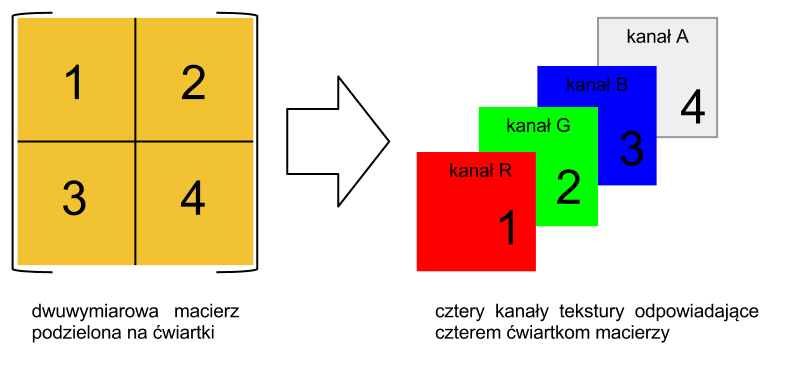
\includegraphics[width=.9\textwidth]{img/rgba14Tex}
\caption{Schemat organizacji danych macierzy NxN w teksturze (N/2)x(N/2)}
\label{fig:rgba14Tex}
\end{figure}

Taki układ danych teoretycznie posiada sporo zalet jak w przypadku użycia
tekstur jednokanałowych. Jednak znacznie zmniejsza on czytelność kodu i
komplikuje implementacje. Utrudnione zostaje przede wszystkim kontrolowanie
warunków brzegowych, programy jednostek cieniujących przetwarzają cztery pola
jednocześnie i stają się bardzo skomplikowane. W przypadku Energy2D komplikacje
programów fragmentów były tak znaczne, że w efekcie odnotowano bardzo słabe
rezultaty pod względem wydajności. Symulacja okazała się być wolniejsza około
34\% od symulacji korzystającej ze schematu RGBA4.

Dlatego też, ostatecznie w Energy2D zastosowano schemat RGBA4. Zapewnia on
stosunkowo dobrą wydajność oraz wsparcie przez większość dostępnych obecnie
urządzeń.